\begin{figure} \centering 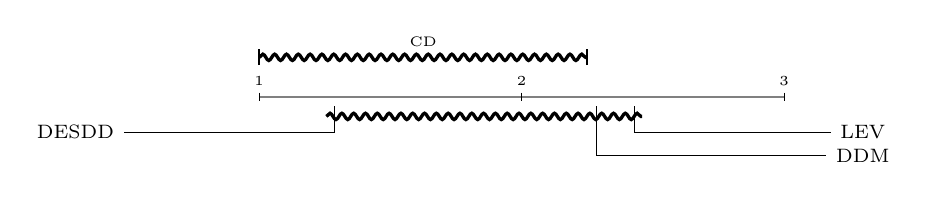
\begin{tikzpicture}[xscale=2]
\node (Label) at  (02.7083,0.7) {\tiny{CD}}; % the label
\draw[decorate,decoration={snake,amplitude=.4mm,segment length=1.5mm,post length=0mm}, very thick, color = black](01.6667, 0.5) -- (03.7500, 0.5);
\foreach \x in {01.6667,03.7500} \draw[thick,color = black] (\x, 0.4) -- (\x, 0.6);

\draw[gray, thick](01.6667, 0) -- (05.0000, 0);
\foreach \x in {01.6667,03.3333,05.0000}\draw (\x cm,1.5pt) -- (\x cm, -1.5pt);
\node (Label) at (01.6667,0.2) {\tiny{1}};
\node (Label) at (03.3333,0.2) {\tiny{2}};
\node (Label) at (05.0000,0.2) {\tiny{3}};
\draw[decorate,decoration={snake,amplitude=.4mm,segment length=1.5mm,post length=0mm}, very thick, color = black](02.0933,-00.2500) -- ( 04.0983,-00.2500);
\node (Point) at (02.1433, 0){};  \node (Label) at (0.5,-00.4500){\scriptsize{DESDD}}; \draw (Point) |- (Label);
\node (Point) at (04.0483, 0){};  \node (Label) at (5.5,-00.4500){\scriptsize{LEV}}; \draw (Point) |- (Label);
\node (Point) at (03.8100, 0){};  \node (Label) at (5.5,-00.7500){\scriptsize{DDM}}; \draw (Point) |- (Label);
\end{tikzpicture}
\caption{desdd_30_95.property}
\label{fig:}
\end{figure}
